
We tested our optimization algorithms by modelling the dive phases and dive types of eleven resident killer whales off the coast of British Columbia, Canada. In addition to testing the performance of our inference methods, the goal of this case study is to jointly infer the dive phases and dive types for resident killer whales in British Columbia.

\subsection{Data Collection and Preprocessing}

The data we use were collected in August and September of 2020 and consist of depth over time. Observations were collected at a rate of 50 Hz using a CATS time-depth recorder, or TDR (Customizable Animal Tracking Solutions, {\em{www.cats.is}}). We down-sampled the depth readings to a frequency of 0.5 Hz. Depth was calibrated using the MATLAB package developed by \citet{Cade:2021}, and a dive was defined as any sequence of depth readings under 0.5 meters that lasted for at least two seconds. The processed data set contains a total of $5858$ dives and $89462$ depth readings. Figure (\ref{fig:data}) shows the depth and change in depth for a subset of dives for one of the whales in the data set. 

\subsection{Model formulation}

Killer whale dive phases may vary between dive types. For example, foraging dives tend to be deeper and longer than resting dives, so it is natural to model the phases of foraging dives differently compared to those of resting dives \citep{Tennessen:2019a}. As such, we use a hierarchical HMM, or HHMM, or jointly model dive types in addition to dive phases \citep{Barajas:2017}. Hierarchical hidden Markov models are specific instances of traditional hidden Markov models, so the machinery developed in this paper is applicable to perform inference. 

We assume that there are three dive types, which is consistent with the harbour porpoises case study examined by \citet{Barajas:2017}. In addition, Researchers are often interested in identifying different phases of dives, in particular the bottom phase of that dive \citep{Wright:2017,}. As such, assume that there are three dive phases per dive type: descent, bottom, and ascent. This results in a total of $N = 9$ hidden states, each corresponding to a different dive phase / dive type combination. 

We set the initial distribution $\delta$ to have the following form:

\begin{equation}
    \delta = \begin{pmatrix} \delta^{(1)} & 0 & 0 & \delta^{(2)} & 0 & 0 & \delta^{(3)} & 0 & 0 \end{pmatrix},
    \label{eqn:delta_case_study}
\end{equation}

since each dive must begin with the descent dive phase. In words, $\delta^{(i)}$ represents the probability that a killer whale begins its dive profile with a dive of type $i$. 

For this hierarchical hidden Markov model, we assume that the transition probability matrix changes over time, so we denote the probability transition matrix as $\Gamma_t$. To this end, we define a coarse-scale transition probability matrix $\Gamma^{(c)} \in \bbR^{3 \times 3}$. For each dive type $i$, we also define a fine-scale probability transition matrix $\Gamma^{(f,i)} \in \bbR^{3 \times 3}$. If an observations occurs \textit{within} a dive, $\Gamma_t$ has a block-diagonal form:

\begin{equation}
    \Gamma_t = 
    \begin{pmatrix}
        \Gamma^{(f,1)} & \mathbf{0} & \mathbf{0} \\
        \mathbf{0} & \Gamma^{(f,2)} & \mathbf{0} \\
        \mathbf{0} & \mathbf{0} & \Gamma^{(f,3)} \\
    \end{pmatrix},
\end{equation}

where $\Gamma^{(f,i)}$ is upper-triangular for $i \in \{1,2,3\}$. The upper-triangular form is selected because the descent and bottom phases of a dive cannot occur after ascent, and the descending phase of a dive cannot occur after bottom.

However, \textit{between} dives, we allow the coarse-scale dive type to transition and force each dive to begin in the descent phase. As such, $\Gamma_t$ takes the following form:
%
\begin{equation}
    \Gamma_t = \Gamma^{(c)} \otimes \begin{pmatrix} 1 & 0 & 0 \\ 1 & 0 & 0 \\ 1 & 0 & 0 \end{pmatrix},
\end{equation}
%
where $\otimes$ denotes the Kronecker product.

Rather than modelling raw depth, we define an observation as the change in depth (in meters) every two seconds. In addition, we model the end of each dive as an observation from the HHMM. We denote an observation as $Y_t = \{D_t,E_t\}$, where $D_t \in \bbR$ is the change in depth in meters and $E_t \in \{0,1\}$ is equal to $1$ if the dive ends at index $t$ and $E_t = 0$ otherwise.

The density of change in depth for dive type $i$ and dive phase $j$ is assumed to follow a normal distribution with mean $\mu^{(i,j)}$ and standard deviation $\sigma^{(i,j)}$, and the probability of the dive ending is assumed to follow a Bernoulli distribution with probability $p^{(i,j)}$. We assume that dives must end on the ascent phase, so we set $p^{(i,1)} = p^{(i,2)} = 0$ for $i = 1,2,3$. Conditioned on the dive type and dive phase, change in depth and the dive end are assumed to be independent.

\subsection{Optimization procedure}

We used a procedure similar to the simulation study to initialize the HMM parameters of the case study. Let $\bar y$ and $s$ denote the sample mean and sample standard deviation of each two-second depth change, respectively. We initialized the mean and standard deviation of the state-dependent density of change in depth as
%
\begin{equation}
    \mu^{(i,j)}_0 \sim \calN(\bar y, s), \quad \log\left(\sigma^{(i,j)}_0\right) \sim \calN(\log(s),1/2), \qquad i,j \in \{1,2,3\},
\end{equation}
%
where $\mu^{(i,j)}_0$ and $\sigma^{(i,j)}_0$ are the initial estimates for mean and standard deviation (respectively) for change in depth within dive type $i$ and dive phase $j$. Further, let $\bar p$ represent the proportion of all two-second observations that occur at the end of a dive. We initialized the state-dependent probability of observing a dive end as
%
\begin{equation}
    p^{(i,1)}_0 = 0, \quad p^{(i,2)}_0 = 0, \quad \logit(p^{(i,3)}_0) \sim \calN(\logit(\bar p),1), \qquad i \in \{1,2,3\},
\end{equation}
%
Where $p^{(i,j)}_0$ is the initial estimate of the probability that a dive will end at a given observation during dive type $i$ and dive phase $j$. Dive phase 3 is ascent.

Let $\eta^{(\delta)}_k$ denote the parameters associated with $\delta$ from equation (\ref{eqn:delta_case_study}) at iteration $k$ of a given optimization algorithm such that

\begin{equation}
    \delta_k^{(i)} = \frac{\exp(\eta^{(\delta,i)})}{\sum_{j=1}^{3} \exp(\eta^{(\delta,j)})}.
\end{equation}

We initialized $\eta^{(\delta)}_0$ as:

\begin{gather}
    \eta_0^{(\delta,1)} = 0, \quad  \eta_0^{(\delta,2)} \sim \calN(0,1), \quad \eta_0^{(\delta,3)} \sim \calN(0,1).
\end{gather}

Let $\eta_k^{(c)} \in \bbR^{3 \times 3}$ denote the parameters associated with the coarse-scale probability transition matrix at iteration $k$ of a given optimization algorithm. The reparameterization from $\eta_k^{(c)}$ to $\Gamma_k^{(c)}$ is given in Equation (\ref{eqn:reparam}). We initialized the diagonal elements of $\eta_0^{(c)}$ as zeros, and we initialized the off-diagonal elements of $\eta_k^{(c)}$ as $\calN(-3,1)$.

Let $\eta_k^{(f,i)} \in \bbR^{3 \times 3}$ denote the parameters associated with fine-scale transition probability matrix $\Gamma_k^{(f,i)}$. The reparameterization from $\eta_k^{(f,i)}$ to $\Gamma_k^{(f,i)}$ is given in Equation (\ref{eqn:reparam}). We initialized all diagonal elements of $\eta_0^{(f,i)}$ as zeros and all off-diagonal elements of $\eta_0^{(f,i)}$ as $\calN(-1,1)$.

%
%If the 2-norm of the average estimated gradient $||\frac{1}{T}\sum_{t=1}^T \widehat \nabla F^{(k,m)}_t + \widehat \nabla G^{(k,m)}_t||$ ever fell below a tolerance of $10^{-8}$, we terminated the M-step of algorithm and moved on to the E-step. Likewise, if the relative change of the log-likelihood after one full E- and M- step of the EM algorithm ever fell below a tolerance of $10^{-10}$, we terminated the algorithm altogether. We found the ground truth MLEs by running the traditional EM algorithm until the relative change in the log-likelihood was on the order of machine precision $10^{-15}$.
%
Similarly to the simulation study, we estimated the parameters of the hierarchical HMM using our six inference algorithms and three baseline algorithms.
%
All algorithms were run using 50 random initializations for a total of 12 hours each on Compute Canada Cedar nodes with 16GB of RAM.

\subsection{Results}
%
\begin{figure}
    \centering
    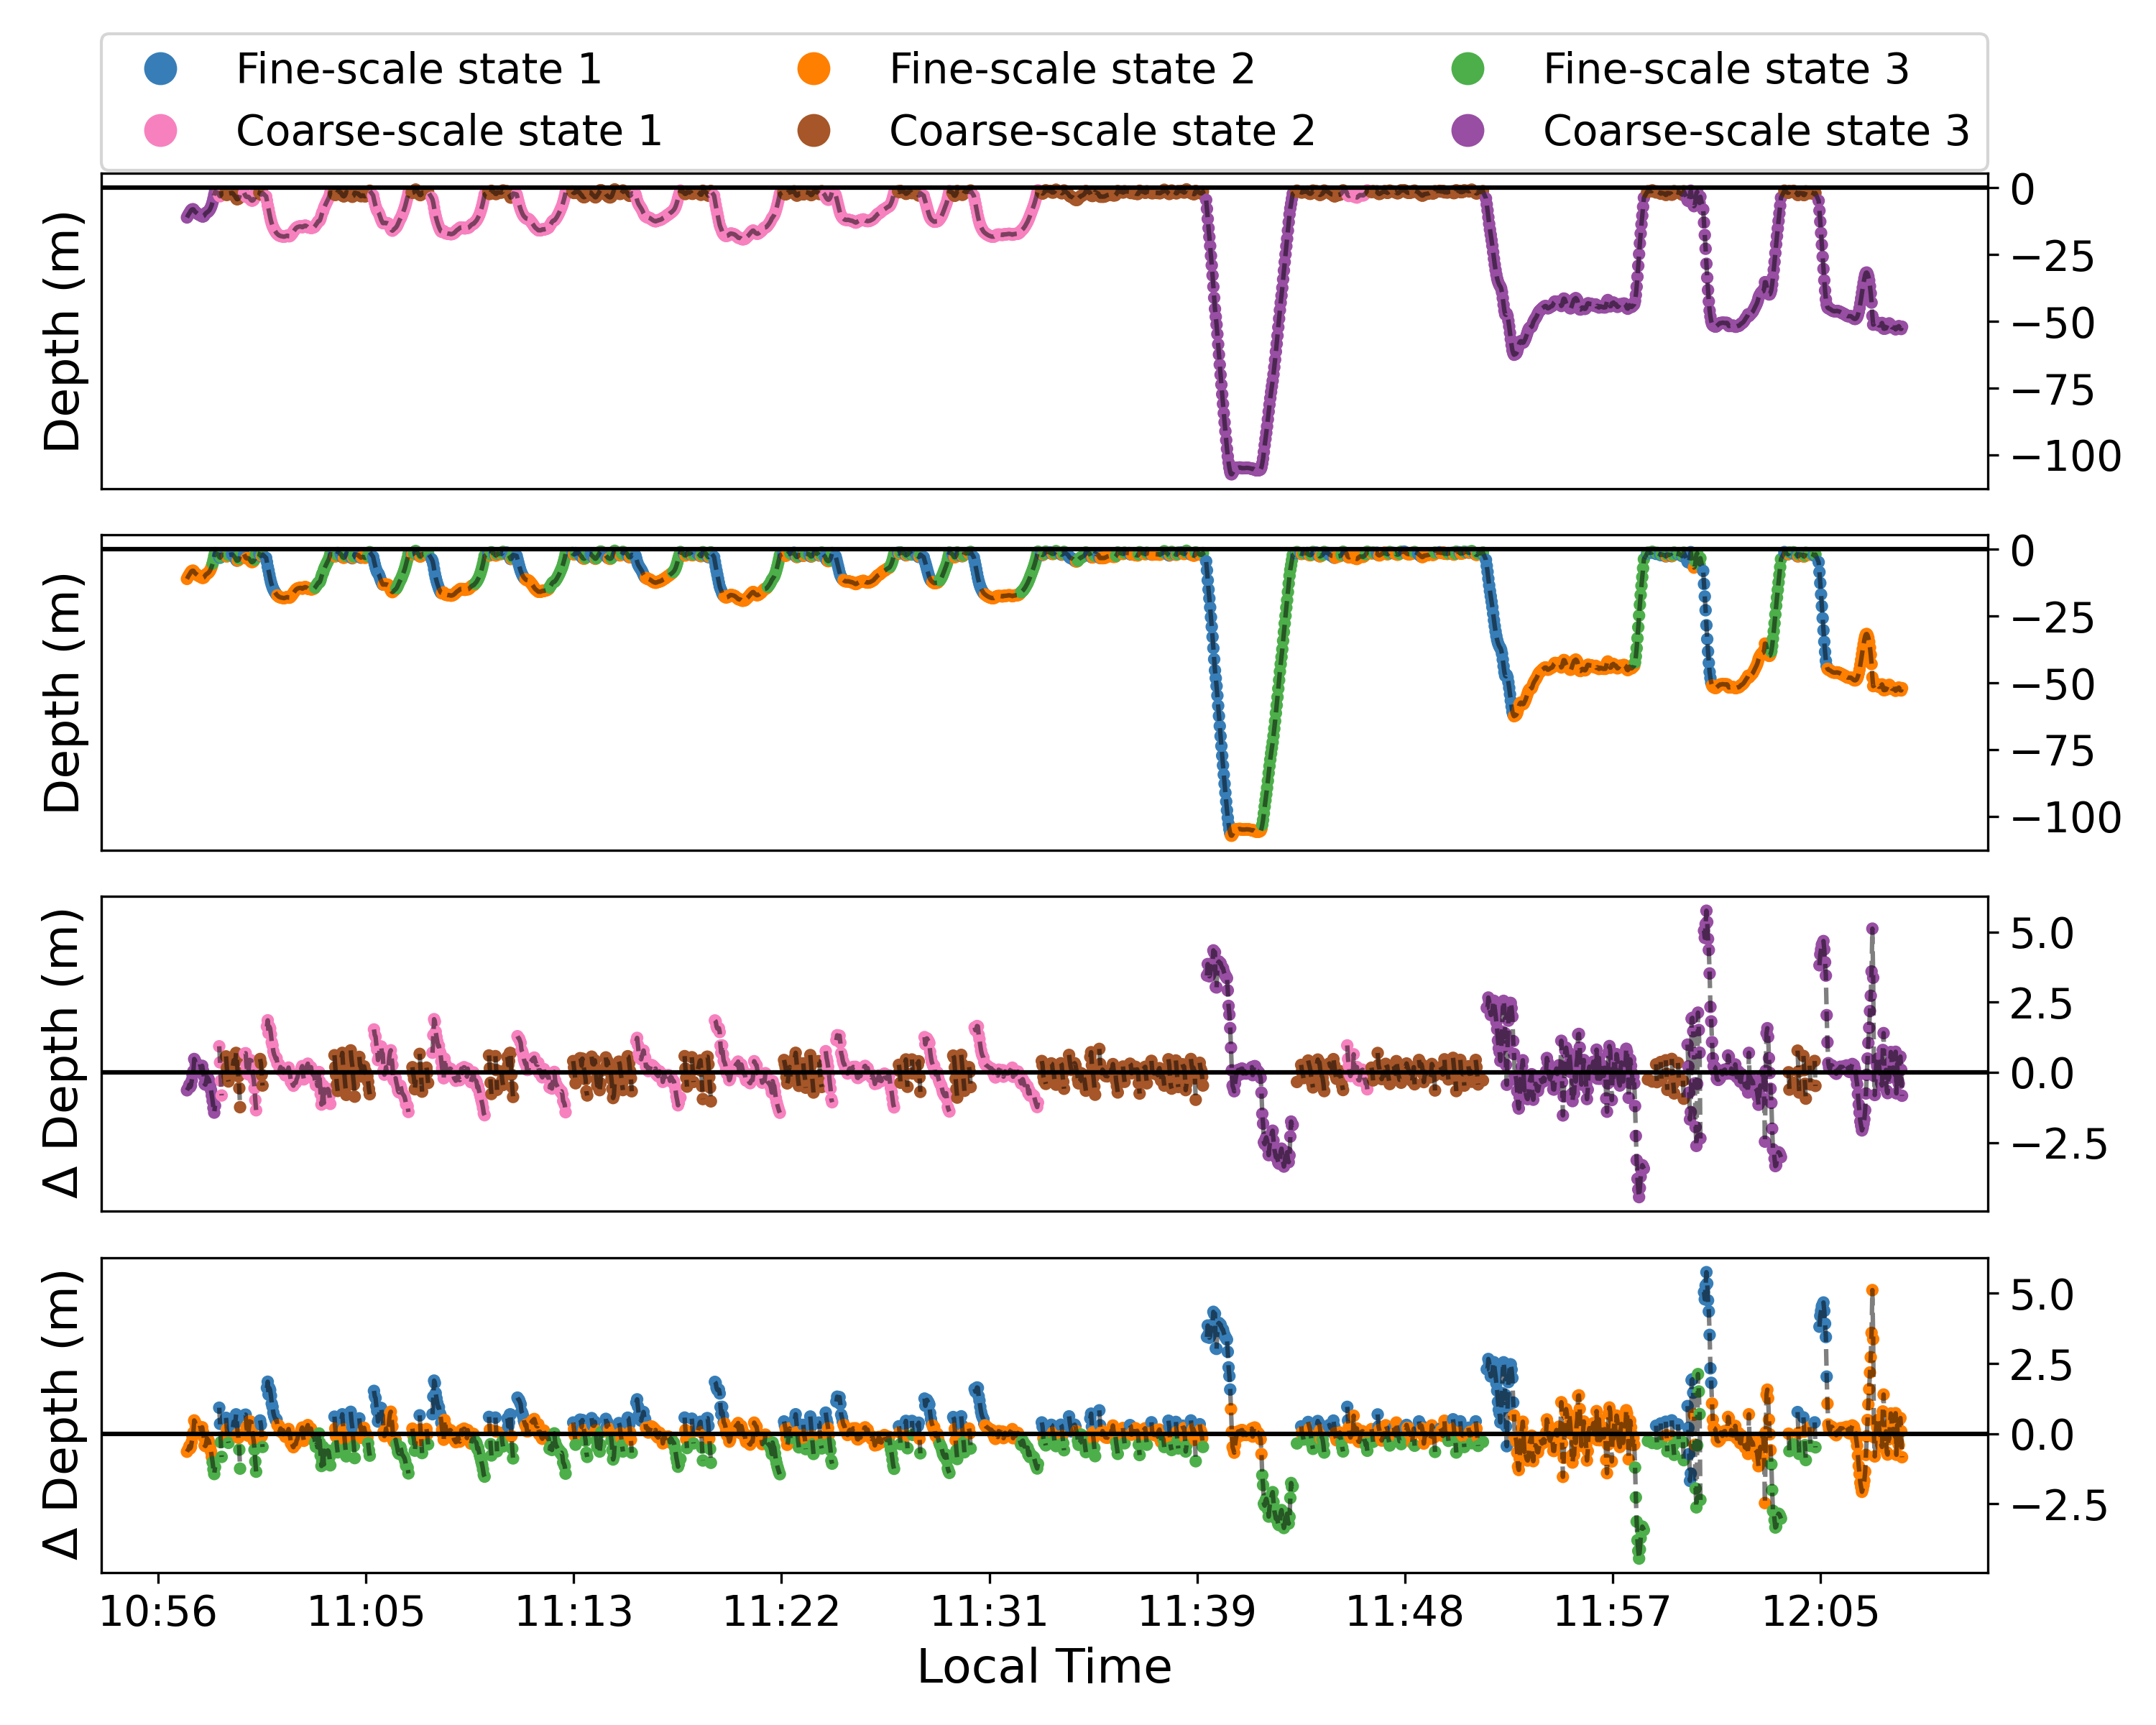
\includegraphics[width=6.5in]{plt/decoded_dives_kw_I107_K_3_3_nWhales_8.png}
    \caption{Depth profile and change in depth associated with a selected Killer whale off the coast of British Columbia, Canada. Data is colour-coded according to the most likely hidden fine-scale state (top three panels) or coarse-scale state (bottom three panels) of each two-second window.}
    \label{fig:data}
\end{figure}
%
Figure (\ref{fig:ll_trace_case}) displays the log-likelihood (divided by $T$) of the maximum log-likelihood minus the log-likelihood (divided by $T$) at each epoch after 12 hours or 100 epochs (whichever came first).
%
\begin{figure}
    \centering
    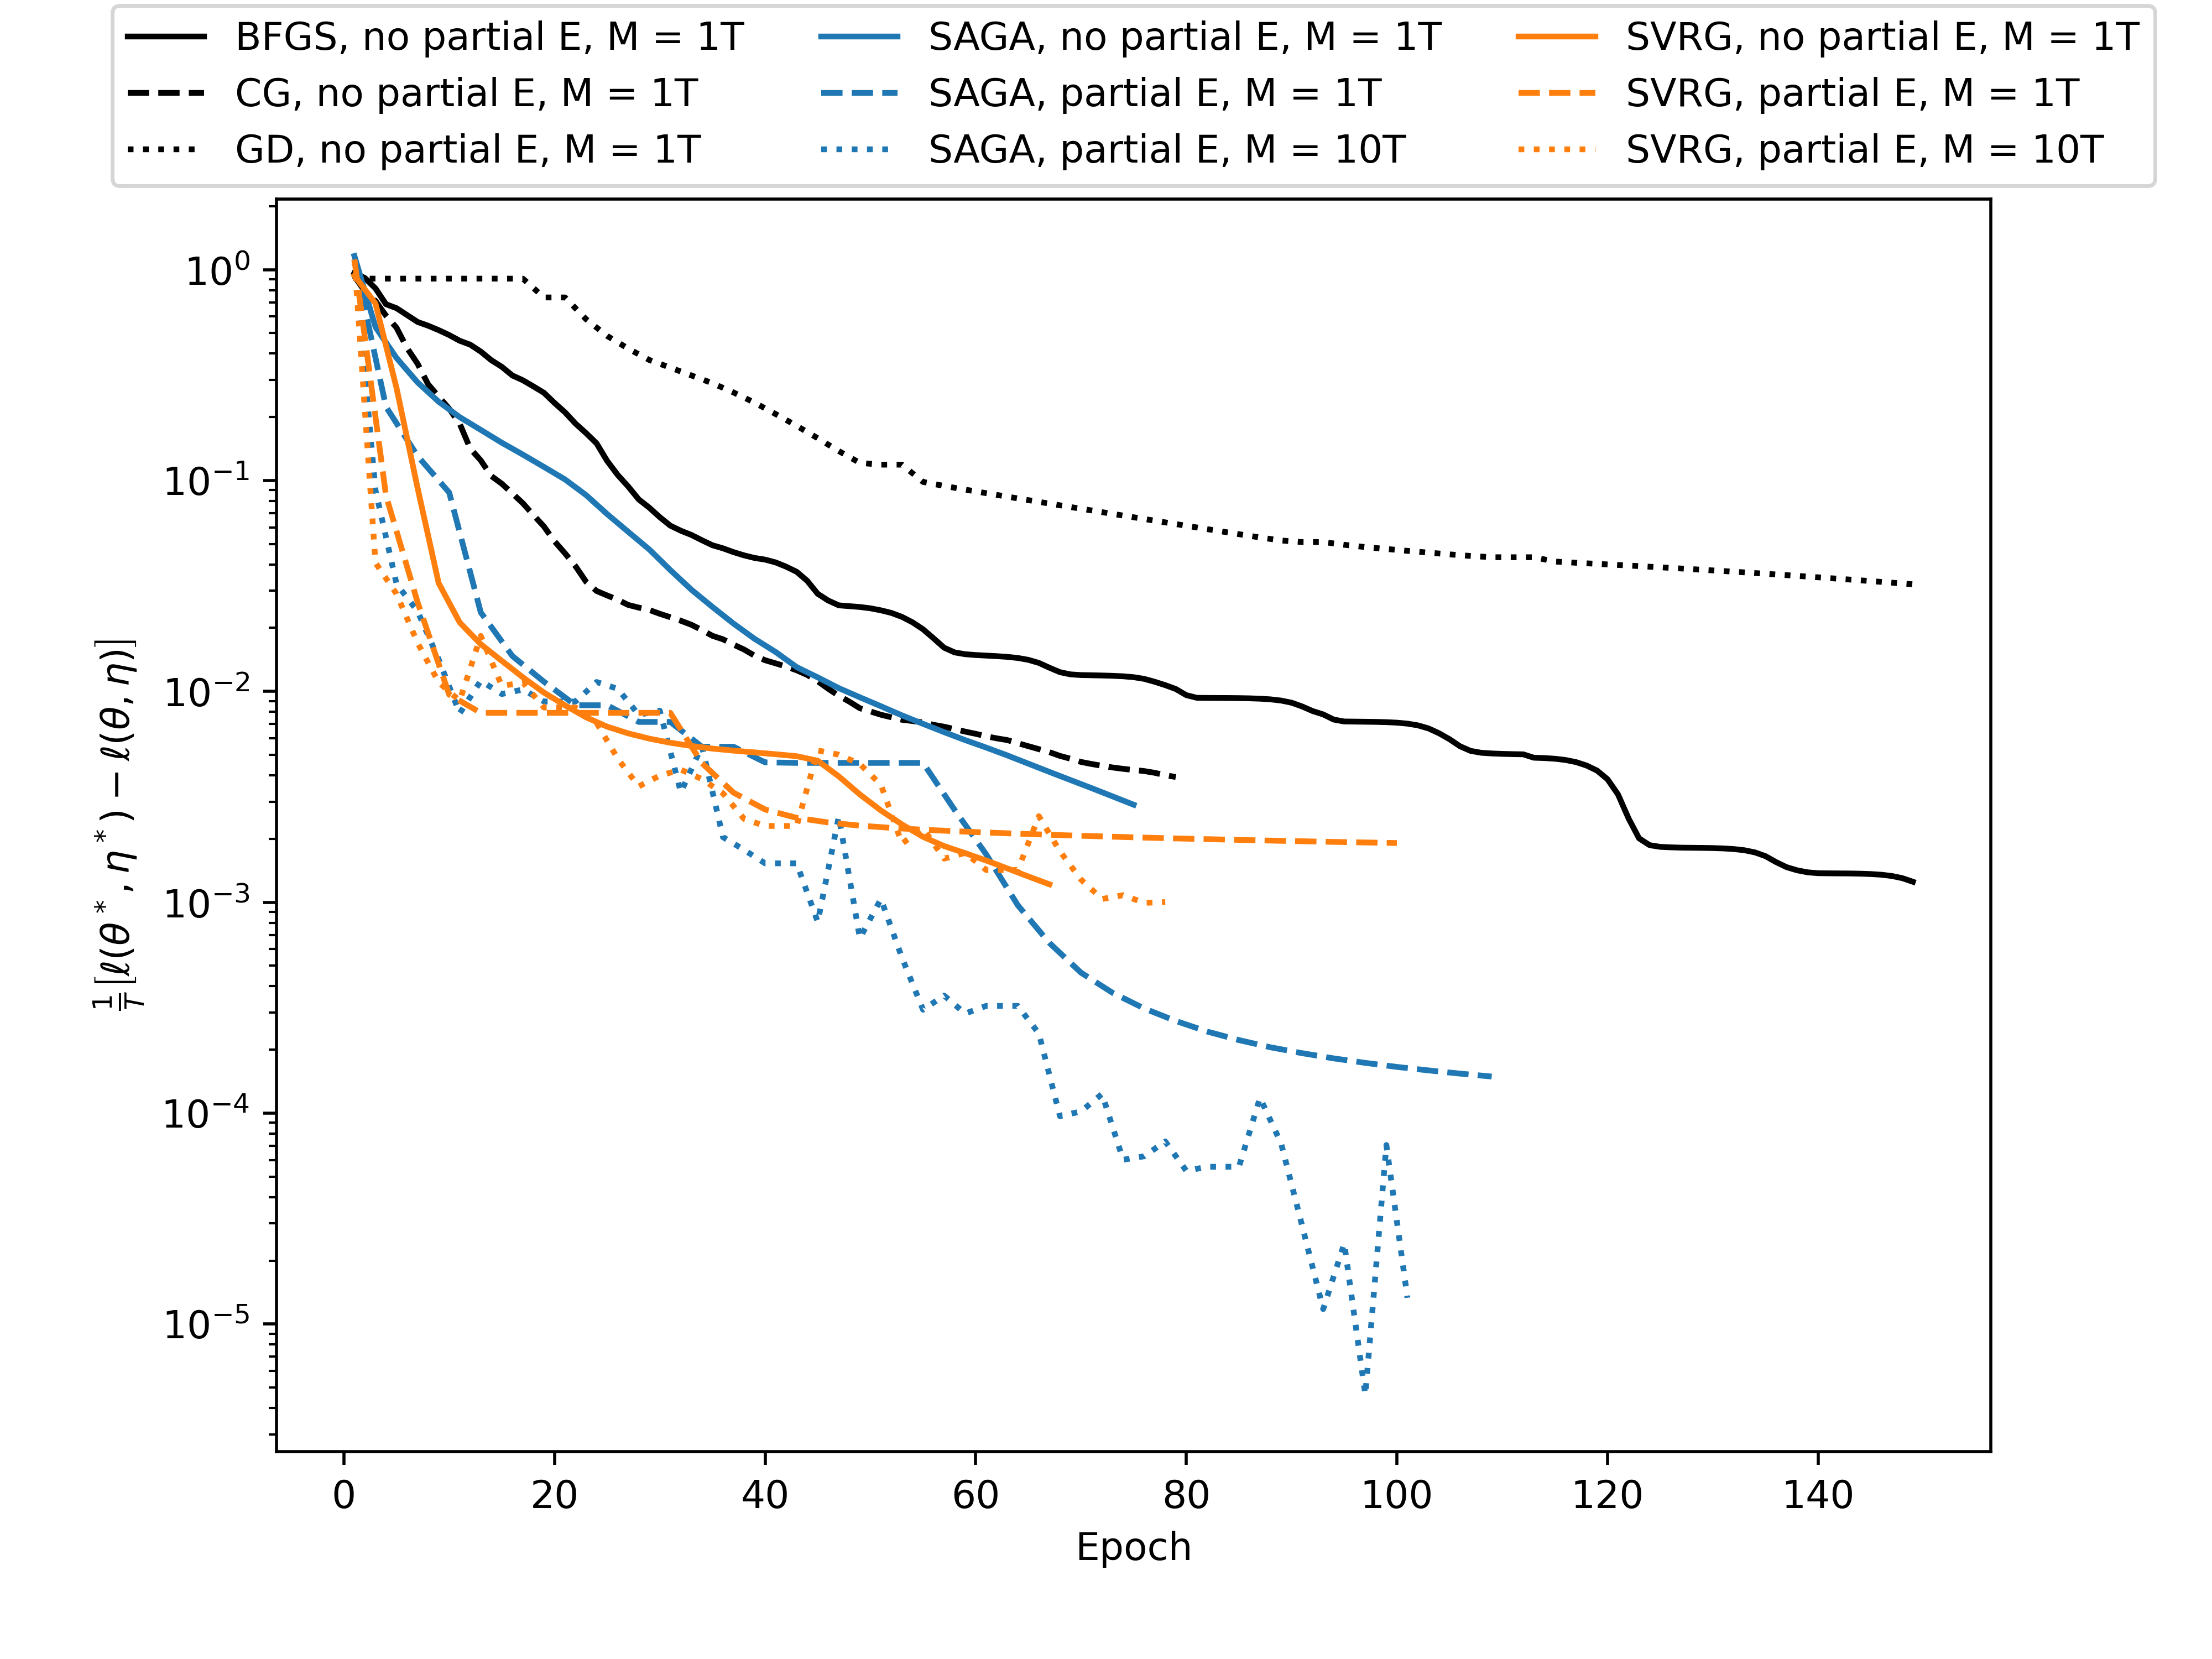
\includegraphics[width=6in]{../plt/log-like_v_epoch_K-3-3.png}
    \caption{Log-likelihood (divided by $T$) of the maximum log-likelihood minus the log-likelihood (divided by $T$) at each epoch after 12 hours or 100 epochs (whichever came first) for the HMM from the Killer Whale case study. For each optimization algorithm, we present the random initialization that resulted in the highest likelihood after 12 hours of computation. The dots correspond to the epoch and likelihood at convergence for each algorithm. Convergence is defined as the point at which the gradient norm of the log-likelihood (divided by $T$) was less than $10^{-2}$. We selected a tolerance of $10^{-2}$ because it was the lowest tolerance that all algorithms regularly converged to within 12 hours. One epoch represents either one full E-step, $T$ iterations with the M-step, or one gradient step for full-gradient algorithms. The y-axis is on a log-scale.}
    \label{fig:ll_trace_case}
\end{figure}
%
Figure (\ref{fig:scatterplot_case}) shows a scatter plot of the loss function (log likelihood divided by $T$) at convergence versus the number of epochs to converge for each random initialization and algorithm.
%
\begin{figure}
    \centering
    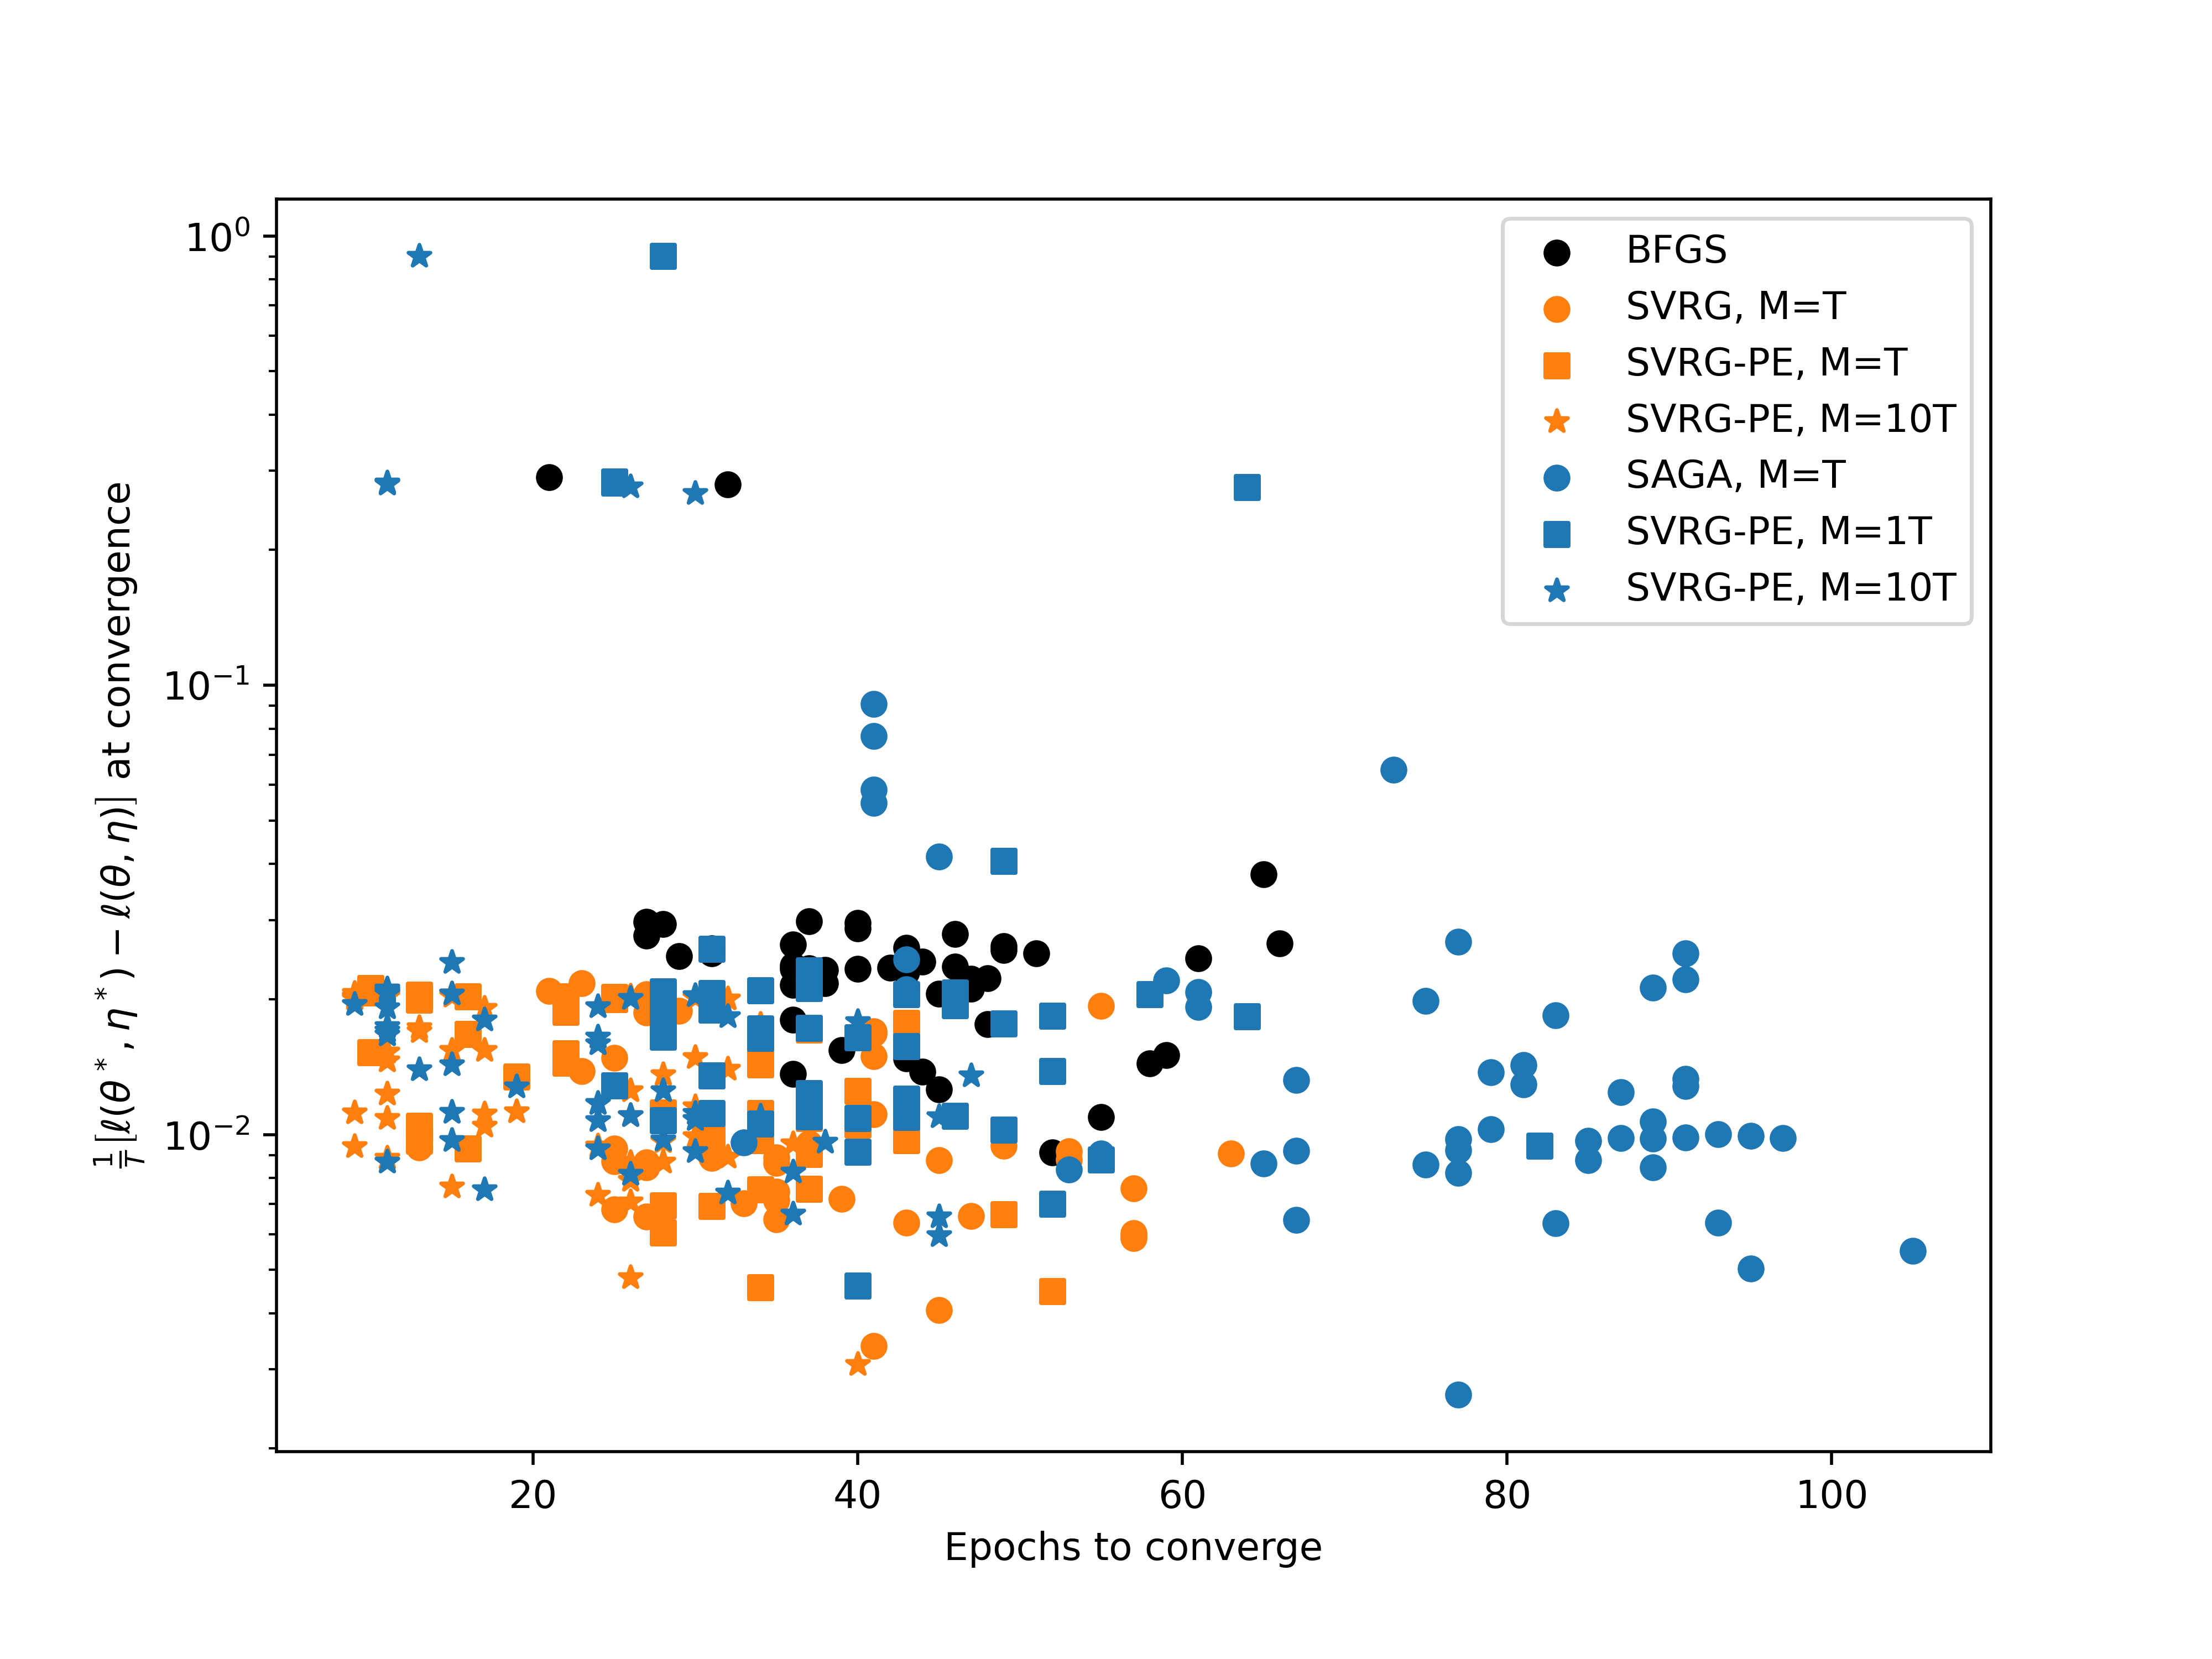
\includegraphics[width=6.5in]{../plt/scatterplot_case_study.png}
    \caption{Log-likelihood of the maximum log-likelihood minus the log-likelihood (all divided by $T$) at convergence versus epochs to converge for the killer whale case study. Convergence is defined as the point at which the gradient norm of the log-likelihood (divided by $T$) was less than $10^{-2}$. We selected a tolerance of $10^{-2}$ because it was the lowest tolerance that all algorithms regularly converged to within 12 hours. One epoch represents either one full E-step, $T$ iterations with the M-step, or one gradient step for full-gradient algorithms. The y-axis is on a log-scale.}
    \label{fig:scatterplot_case}
\end{figure}

Like the simulation study, SVRG tended to converge in fewer epochs compared to SAGA for all stochastic algorithms. In addition, all stochastic algorithms converged in fewer epochs and to regions of higher likelihood compared to the full-batch baselines (BFGS and conjugate gradient). SVRG with a partial E step and $M=T$ tended to converge in the fewest epochs to regions of high likelihood (see Figure (\ref{fig:scatterplot_case})), but all algorithms converged to regions of high likelihood with varying reliability. The partial E step algorithms (Algorithm \ref{alg:P-EM-SO}) appear to be of particular use early on in the optimization procedure (i.e the first ~ 5 epochs). This is intuitive because the proper weights ($\gamma$ and $\xi$) change rapidly early in the optimization procedure.

%All of the algorithms presented in this paper converge with higher likelihood than BFGS (on average), and all algorithms except for algorithm (\ref{alg:P-EM-SO}) with SAGA tend to converge in fewer epochs than BFGS.

%Figure (\ref{fig:scatter_case}) displays scatter plots of the number of epochs to converge and the loss at convergence of each algorithm vs. BFGS for the same data set and parameter initializations.
%
%\begin{figure}
%    \centering
%    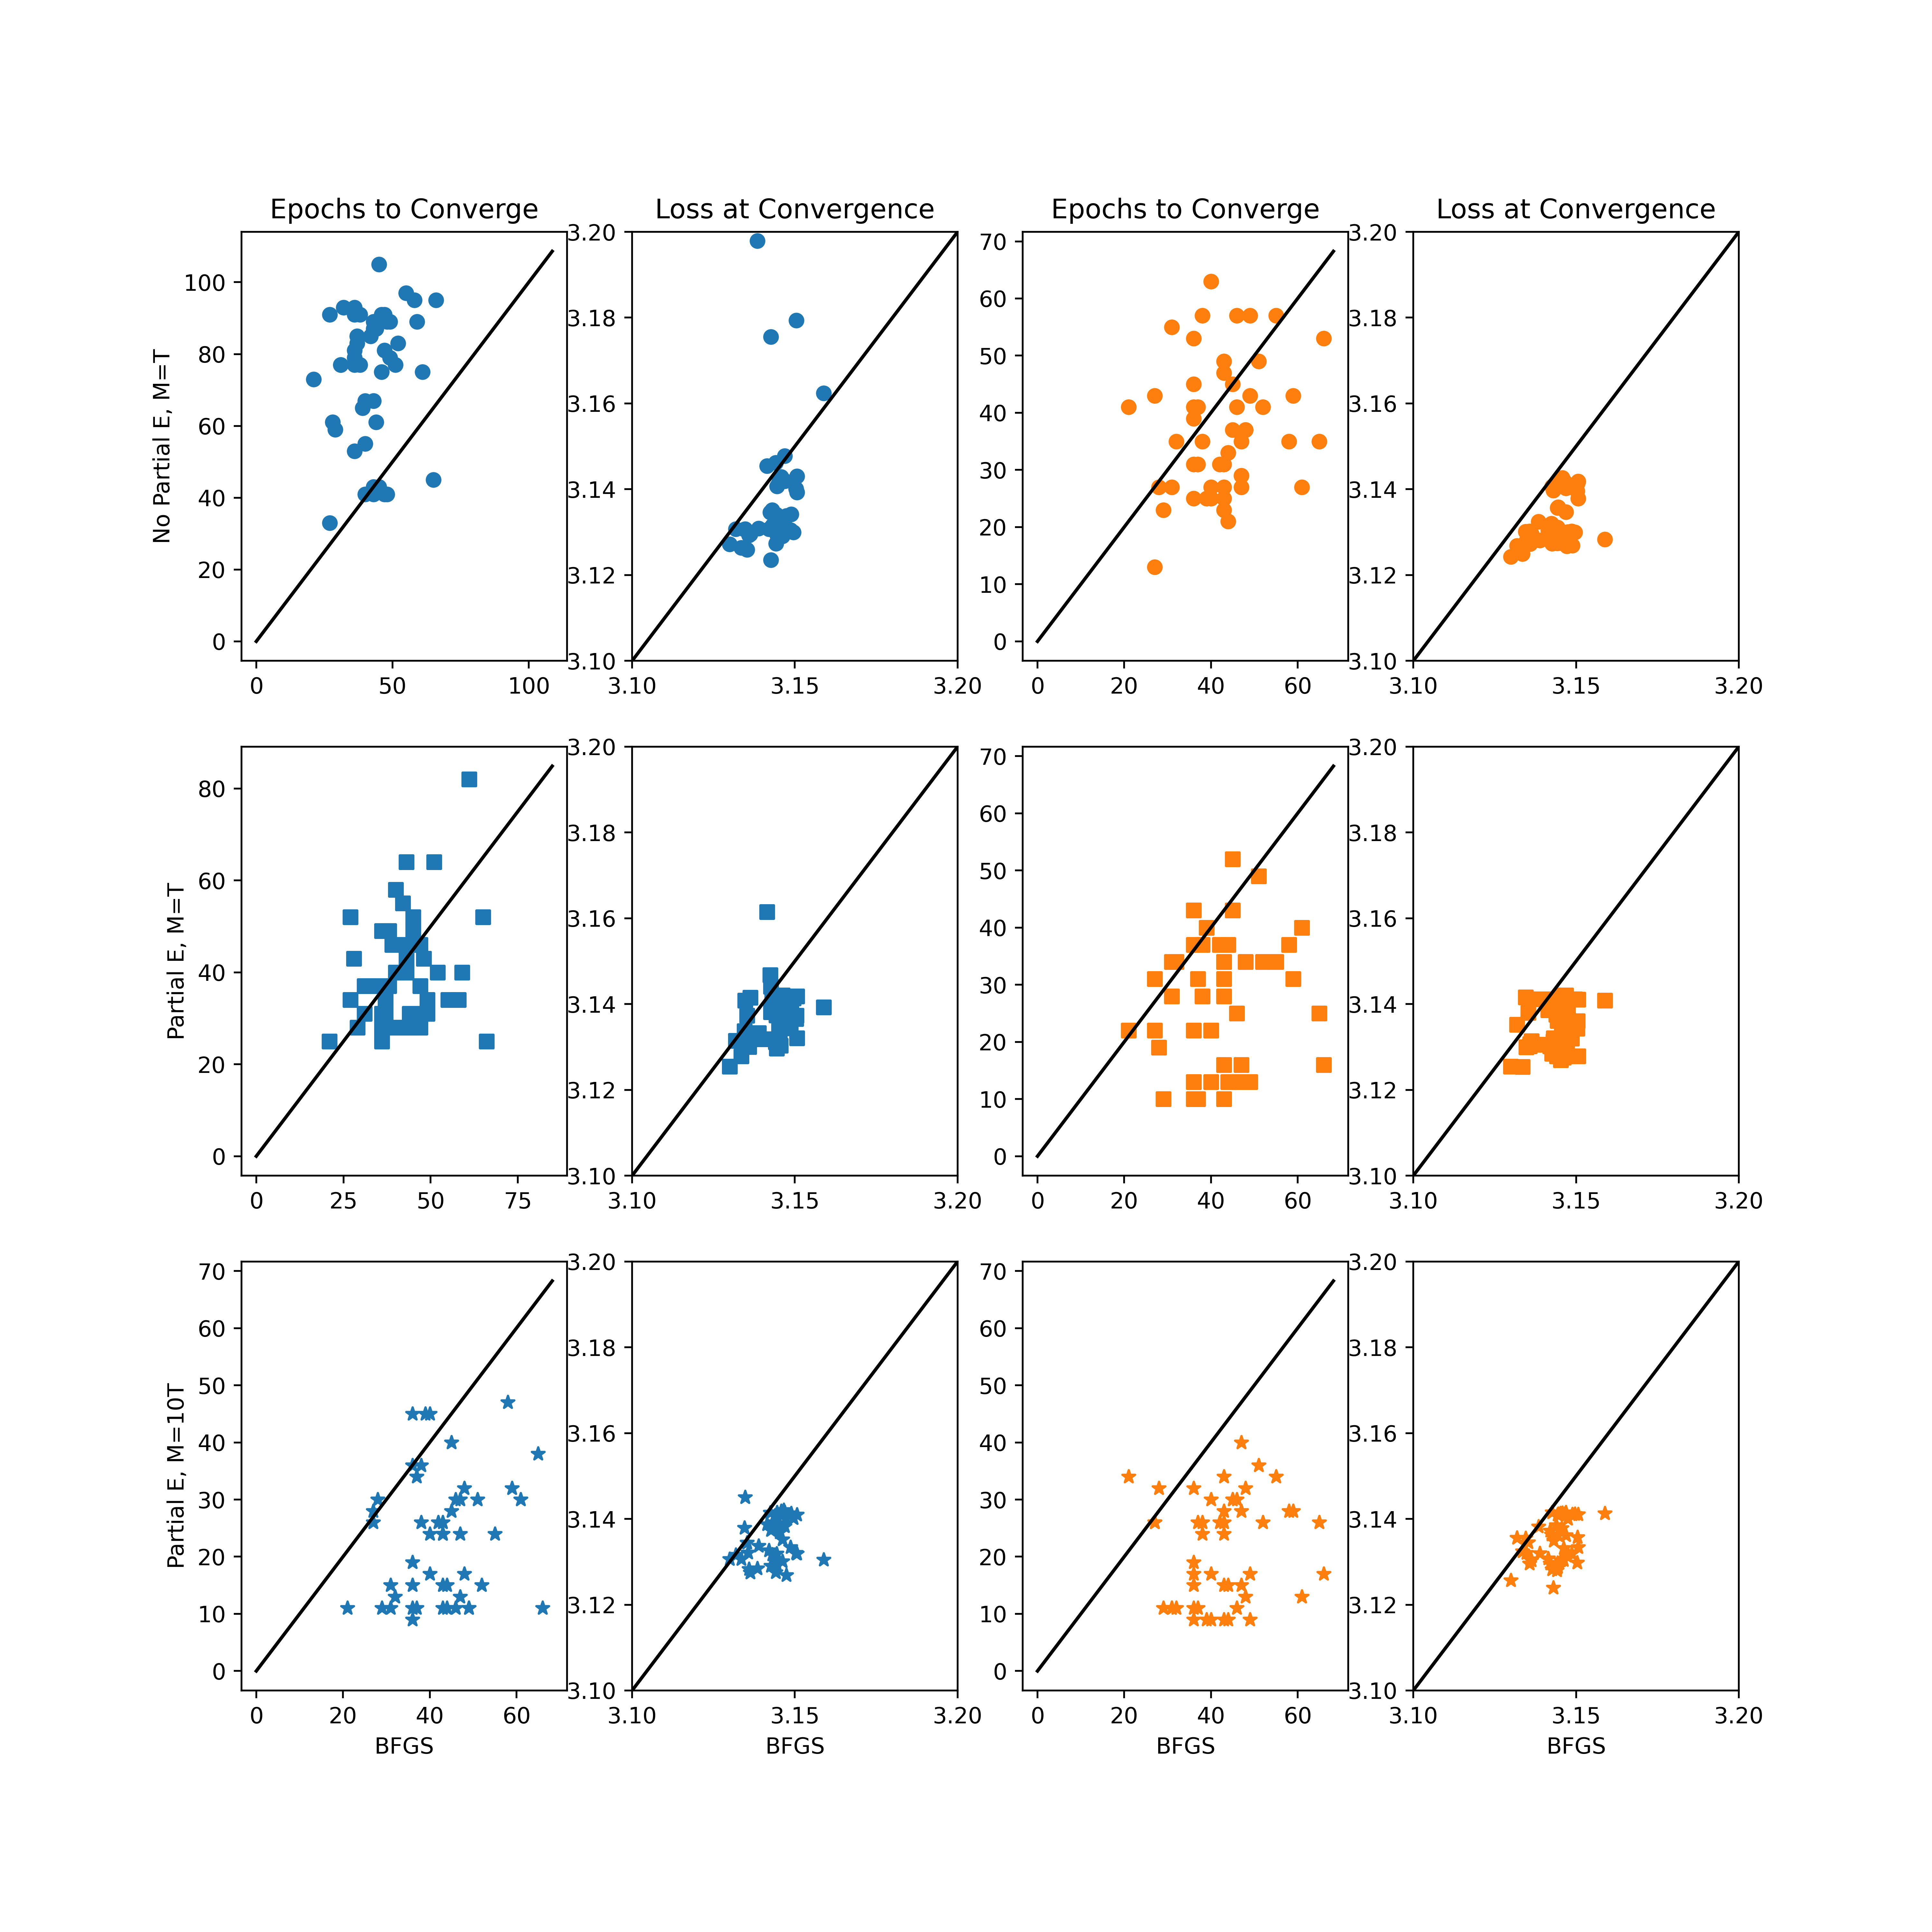
\includegraphics[width=6.5in]{../plt/paired_scatter_case_study.png}
%    \caption{Number of epochs to converge (columns 1 and 3) and the loss at convergence (columns 2 and 4) of each algorithm vs. BFGS for identical data sets and parameter initializations. Lower is better for both criteria, so data points below the line $y=x$ suggest that the stochastic optimization algorithms perform better.}
%    \label{fig:scatter_case}
%\end{figure}
%

%SAGA without a partial E-step performs similarly to the EM algorithm in a per-epoch basis because SAGA is successfully converging for the M-step when $M = T$. However, it does not perform as well as the EM algorithm on a per-time basis because the M-step is significantly slower when using SAGA vs the closed-form solution. This behaviour is expected, and SAGA has a significant advantage over the EM algorithm in that it only requires gradients rather than sufficient statistics.

%mplementing a partial E-step shows that SAGA can outperform the EM algorithm when the parameter estimates are far from the optimal solutions and when the underlying HMM does not mix rapidly. This is likely because the weights of the $F$ and $G$ are very inaccurate at first, and updating them early in the optimization procedure yields a significant speed-up. In addition, if the Markov chain is rapidly mixing, then updates to $\gamma_{t_m}$ and $\xi_{t_m}$ at a single data point are more accurate. Future work may involve performing the partial-E step for many weights at once sequentially, depending upon the mixing time of the current estimate of $\eta_k$.